\begin{figure}[!htbp]
    % Row 1
    \def\subfigheight{1.8cm}
    \begin{subfigure}[t]{0.295\textwidth}
        %\includesvg[inkscapelatex=false, height=\subfigheight]{new_instances/inverted/final_best_gardeyn0.svg}
        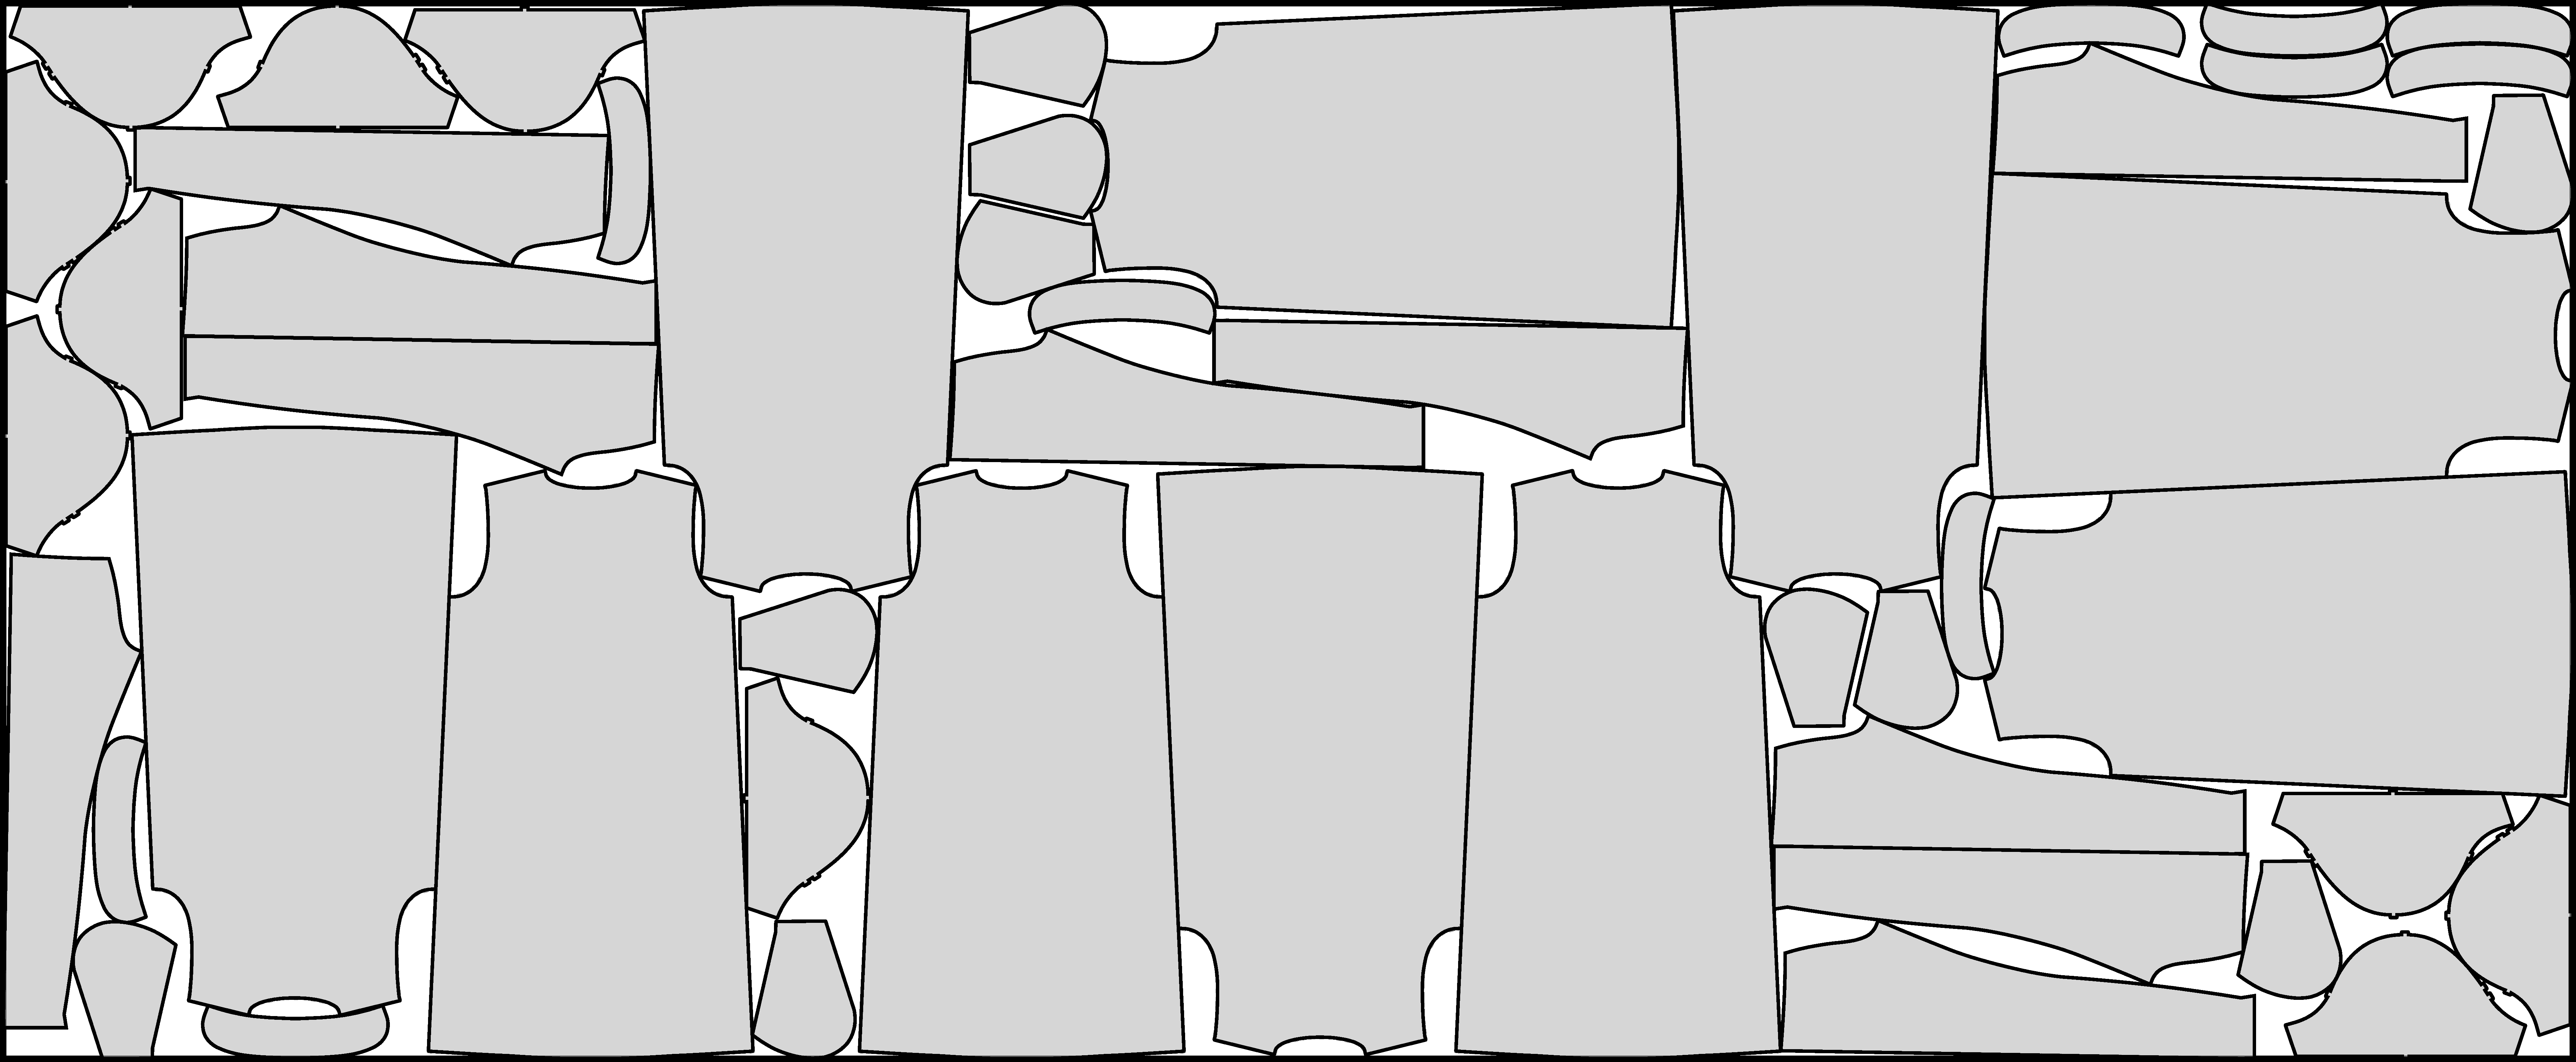
\includegraphics[height=\subfigheight]{final_best_gardeyn0_svg-raw.pdf}
        \caption{\texttt{GARDEYN0}}
    \end{subfigure}
    \hfill
    \begin{subfigure}[t]{0.12\textwidth}
        \centering
        %\includesvg[inkscapelatex=false, height=\subfigheight]{new_instances/inverted/final_best_gardeyn1.svg}
        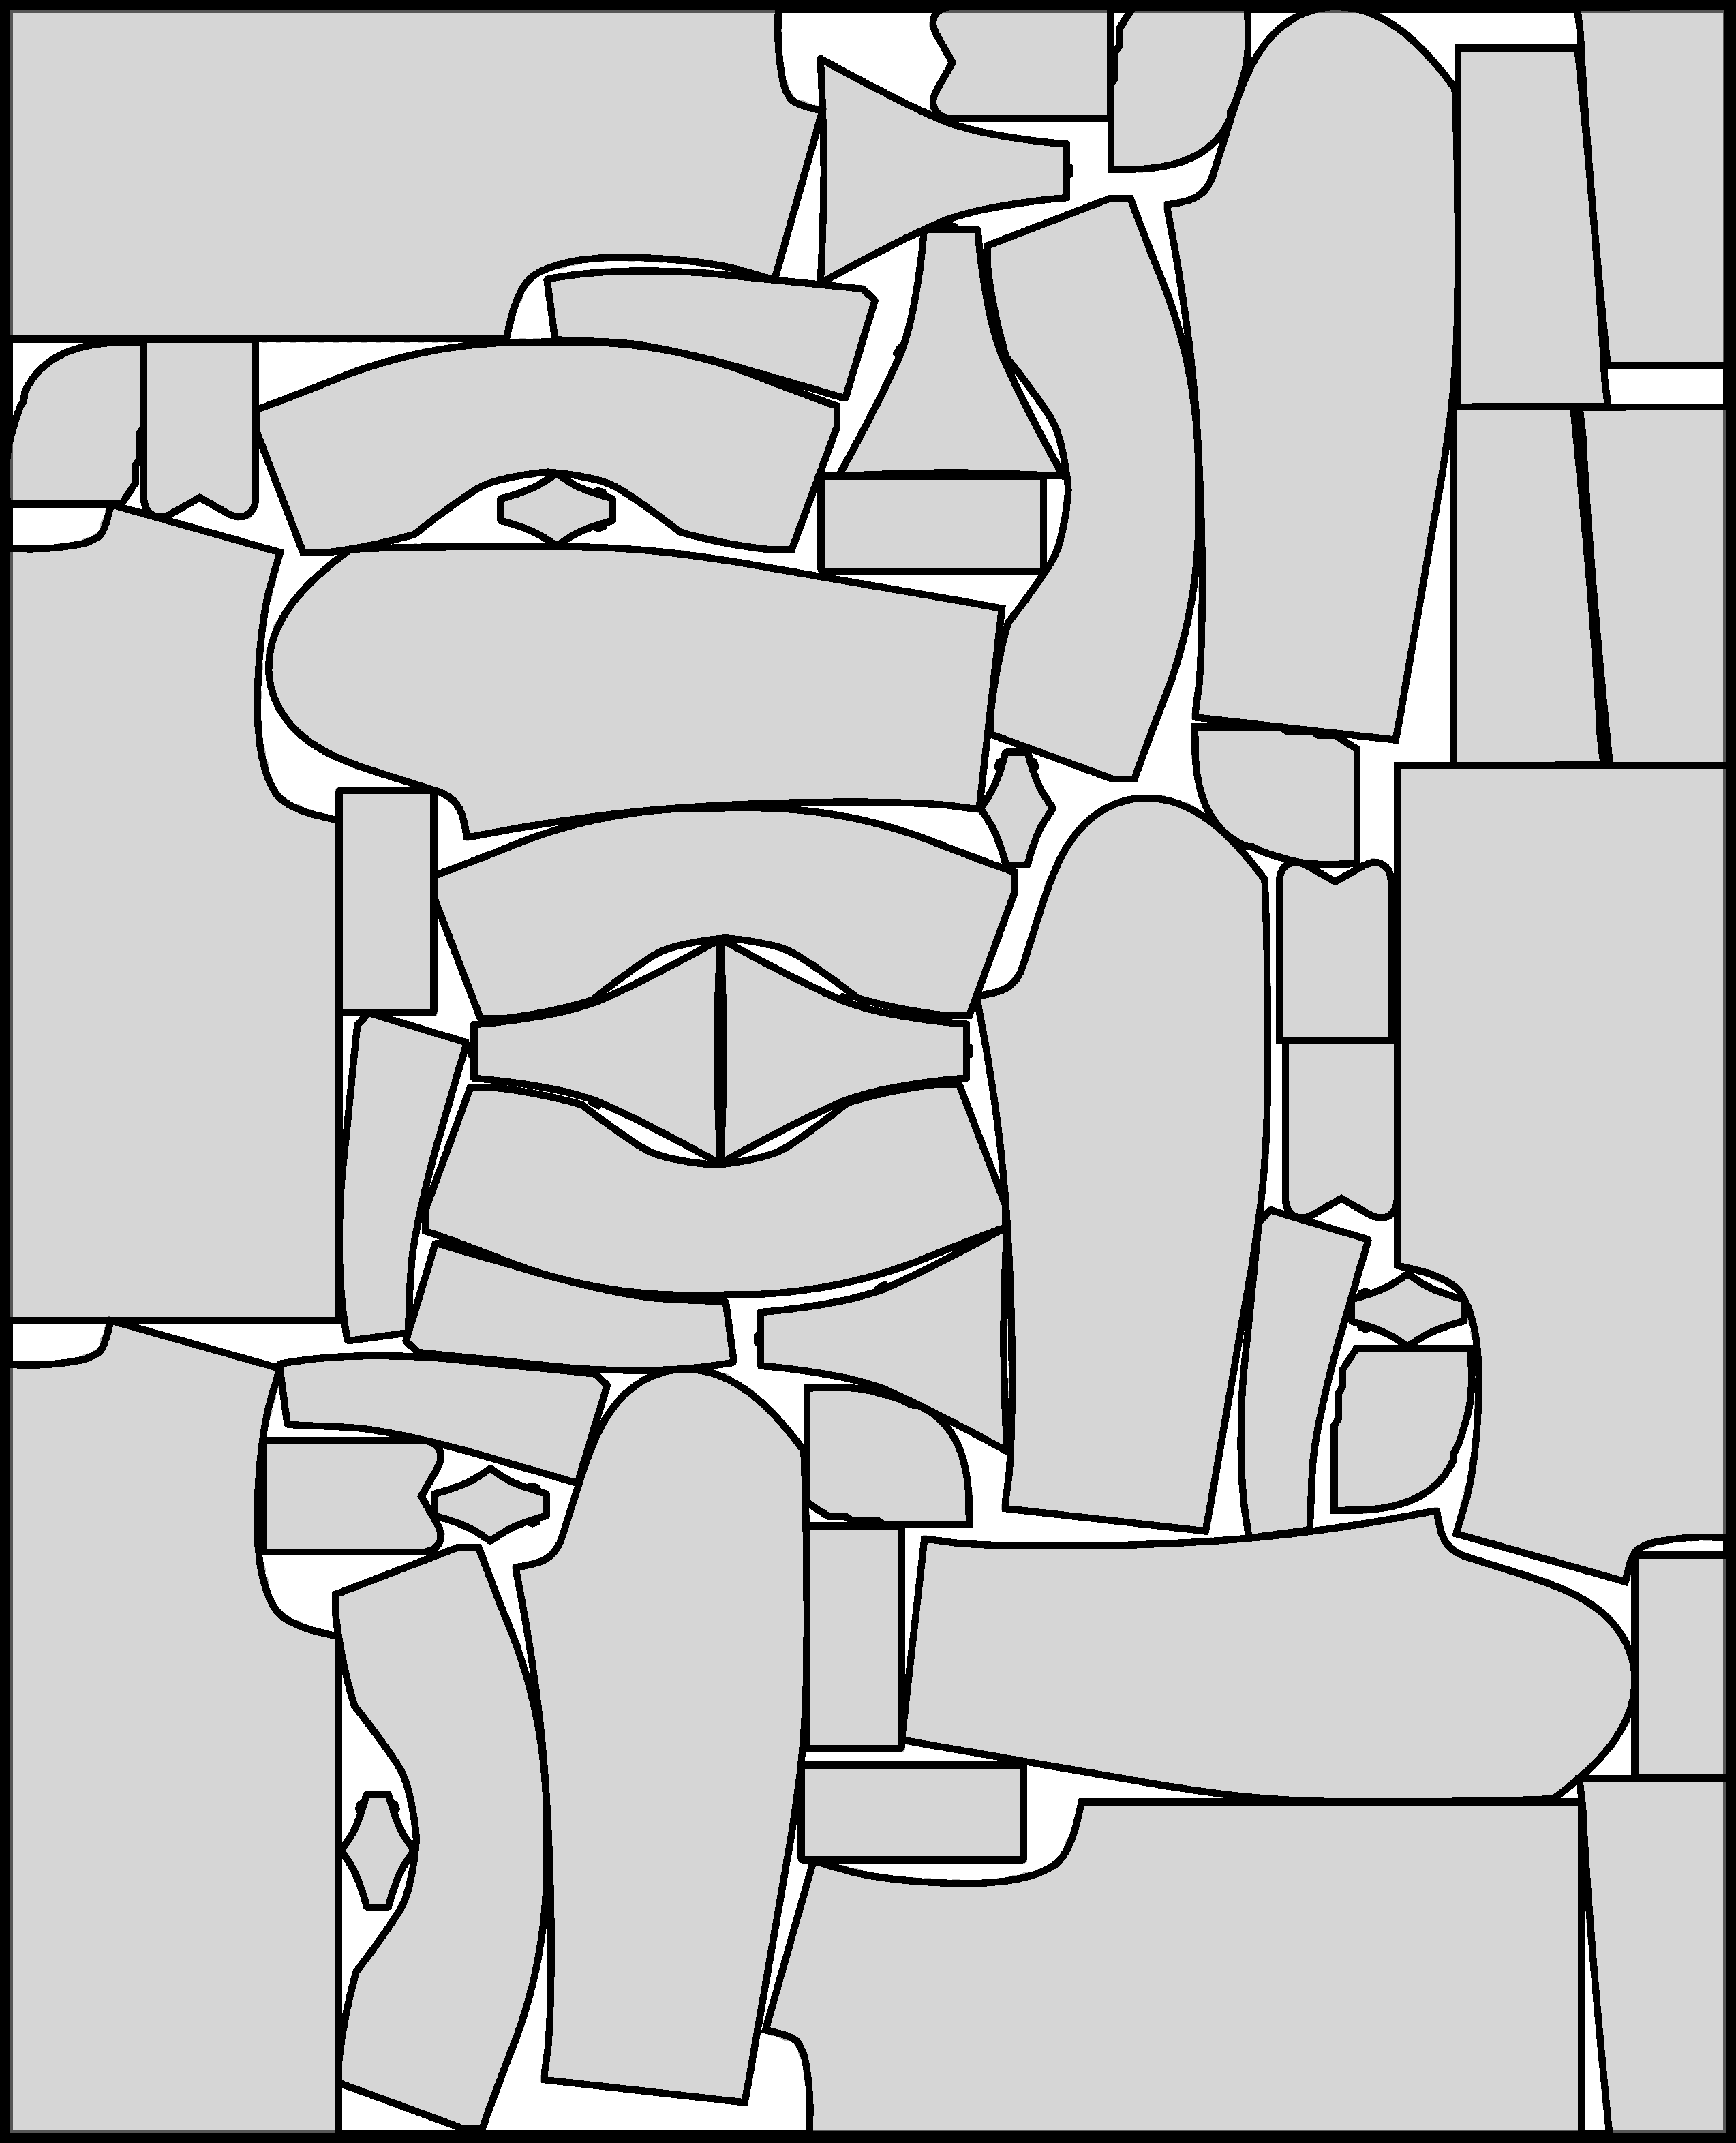
\includegraphics[height=\subfigheight]{final_best_gardeyn1_svg-raw.pdf}
        \caption{\texttt{GARDEYN1}}
    \end{subfigure}
    \hfill
    \begin{subfigure}[t]{0.57\textwidth}
        \hfill
        %\includesvg[inkscapelatex=false, height=\subfigheight]{new_instances/inverted/final_best_gardeyn2.svg}
        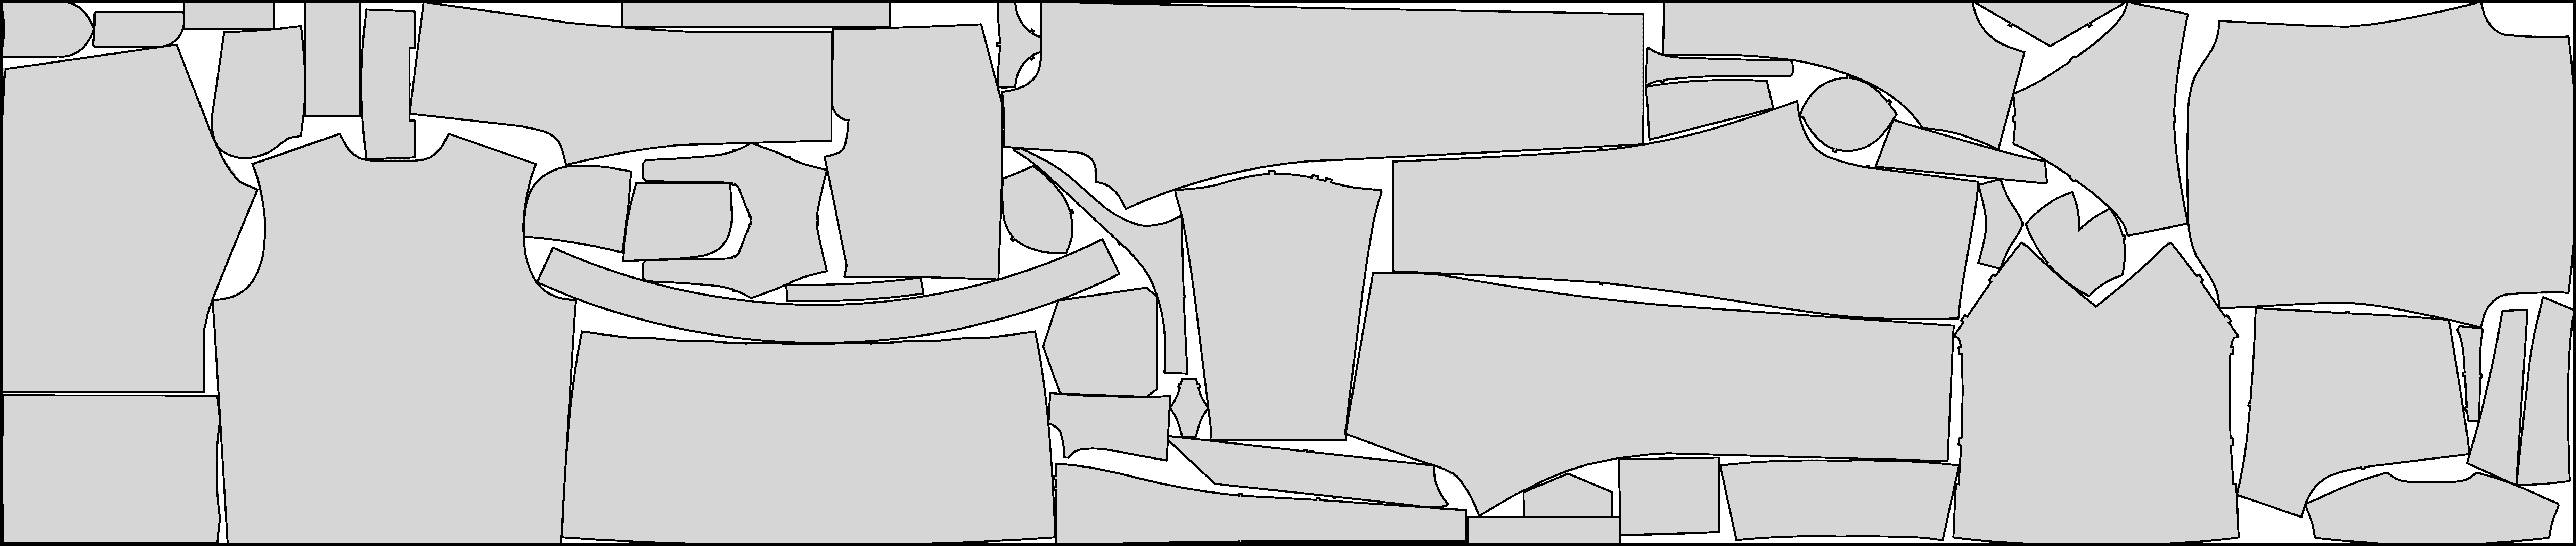
\includegraphics[height=\subfigheight]{final_best_gardeyn2_svg-raw.pdf}
        \caption{\texttt{GARDEYN2}}
    \end{subfigure}

    \vspace{.5em}
        
    \def\subfigheight{2.4cm}
    \begin{subfigure}[t]{0.48\textwidth}
        %\includesvg[inkscapelatex=false, height=\subfigheight]{new_instances/inverted/final_best_gardeyn3.svg}
        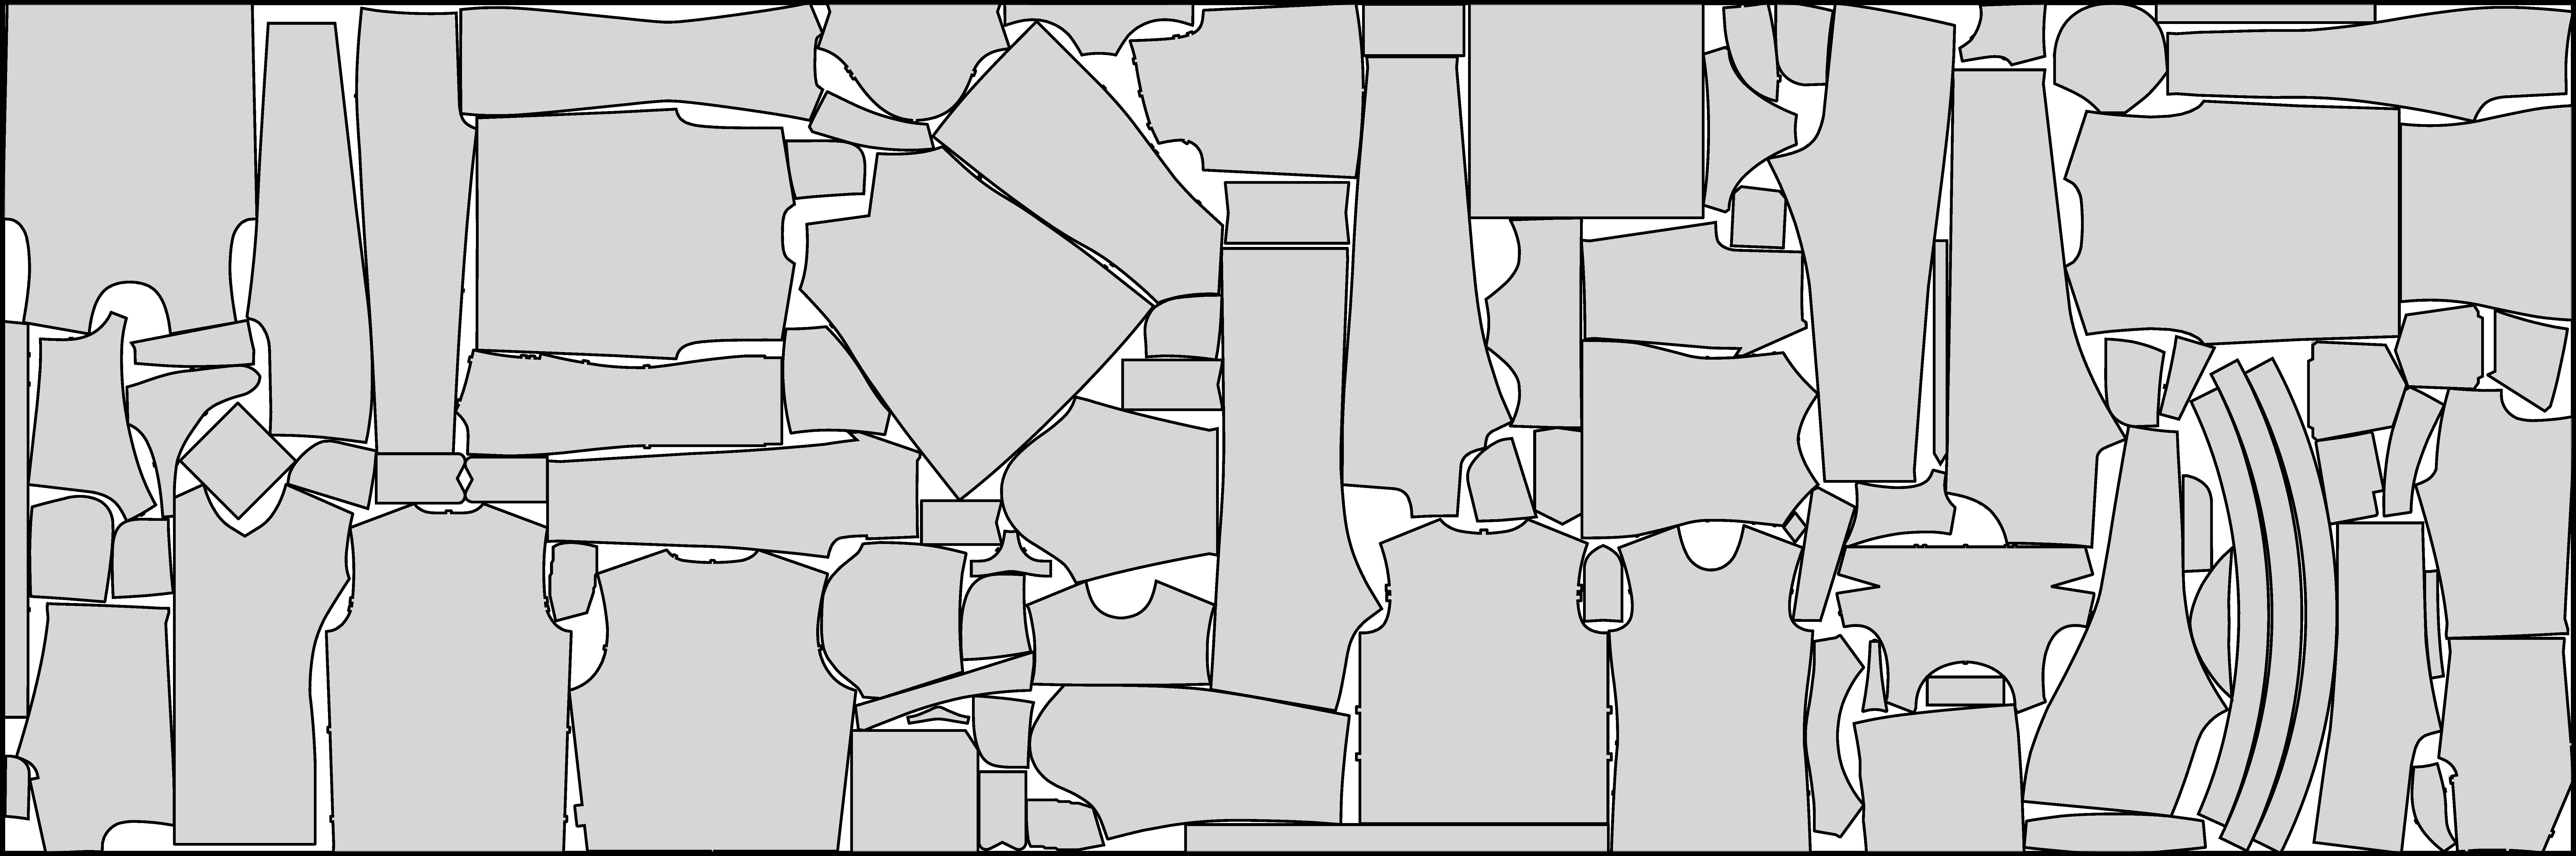
\includegraphics[height=\subfigheight]{final_best_gardeyn3_svg-raw.pdf}
        \caption{\texttt{GARDEYN3}}
    \end{subfigure}
    \hfill
    \begin{subfigure}[t]{0.51\textwidth}
        \hfill
        %\includesvg[inkscapelatex=false, height=\subfigheight]{new_instances/inverted/final_best_gardeyn4.svg}
        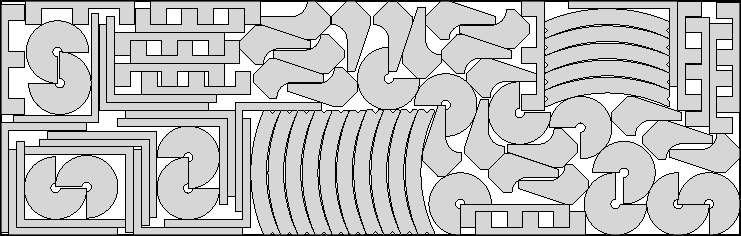
\includegraphics[height=\subfigheight]{final_best_gardeyn4_svg-raw.pdf}
        \caption{\texttt{GARDEYN4}}
    \end{subfigure}

    \vspace{.5em}

    \def\subfigheight{2.3cm}
    \begin{subfigure}[t]{0.33\textwidth}
        %\includesvg[inkscapelatex=false, height=\subfigheight]{new_instances/inverted/final_best_gardeyn5.svg}
        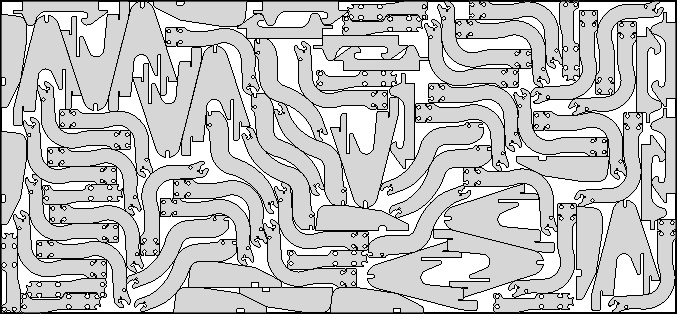
\includegraphics[height=\subfigheight]{final_best_gardeyn5_svg-raw.pdf}
        \caption{\texttt{GARDEYN5}}
    \end{subfigure}
    \hfill
    \begin{subfigure}[t]{0.65\linewidth}
        \hfill
        %\includesvg[inkscapelatex=false, height=\subfigheight]{new_instances/inverted/final_best_gardeyn6.svg}
        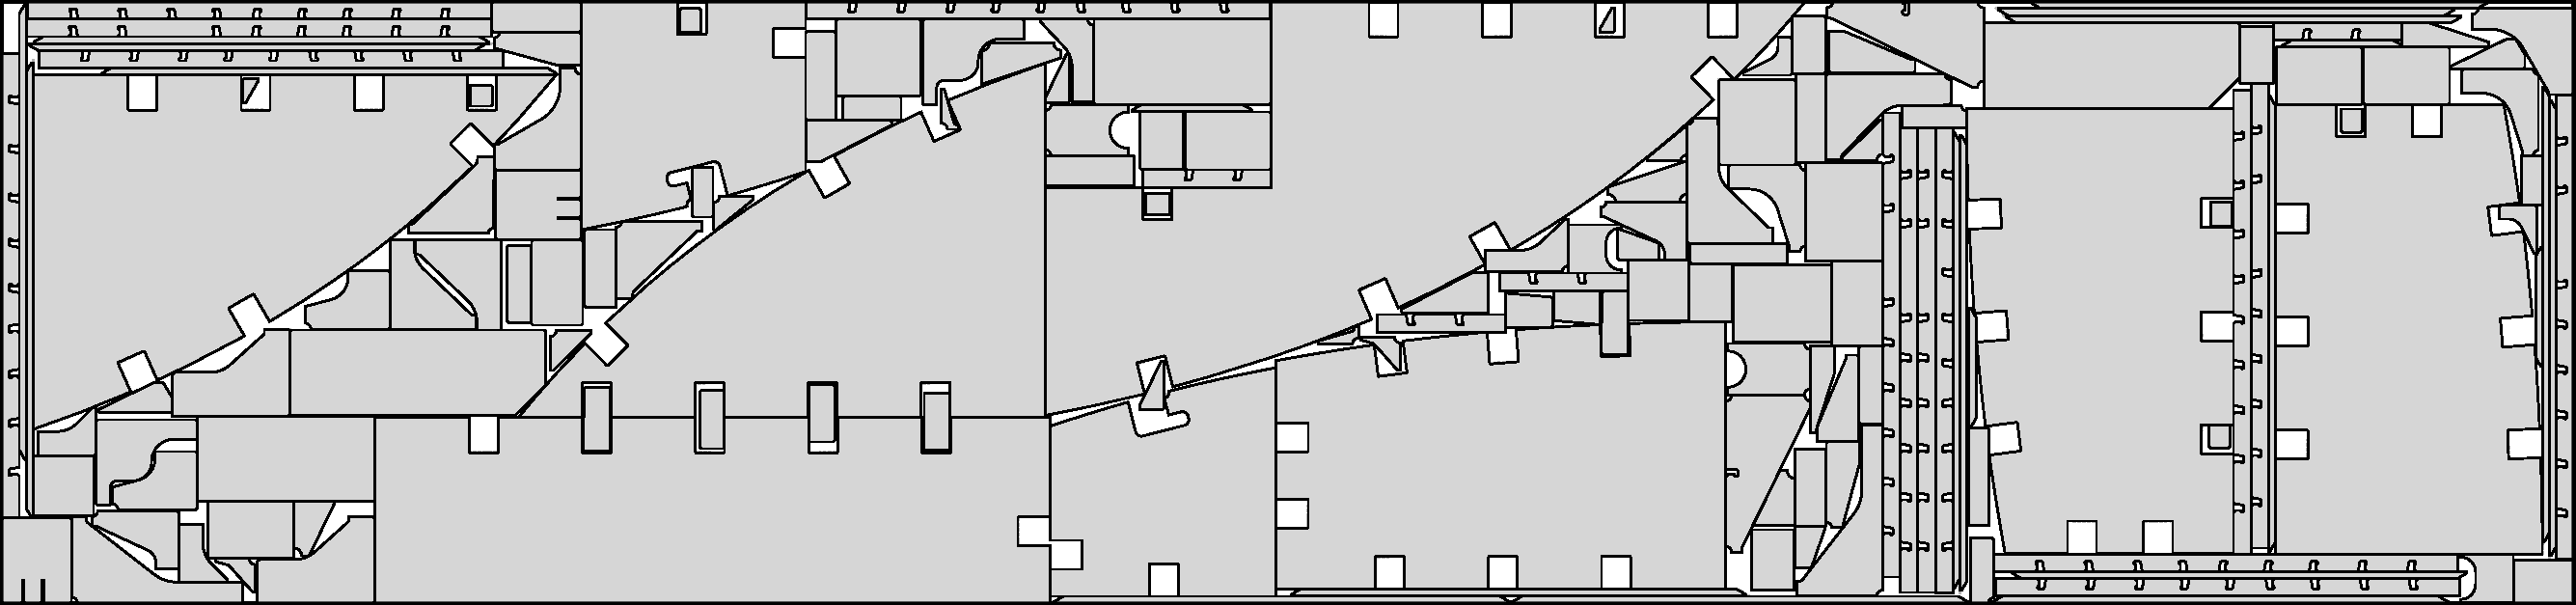
\includegraphics[height=\subfigheight]{final_best_gardeyn6_svg-raw.pdf}
        \caption{\texttt{GARDEYN6}}
    \end{subfigure}
    
    \vspace{.5em}

    \def\subfigheight{2cm}

    \begin{subfigure}[t]{0.44\linewidth}
        %\includesvg[inkscapelatex=false, height=\subfigheight]{new_instances/inverted/final_best_gardeyn7.svg}
        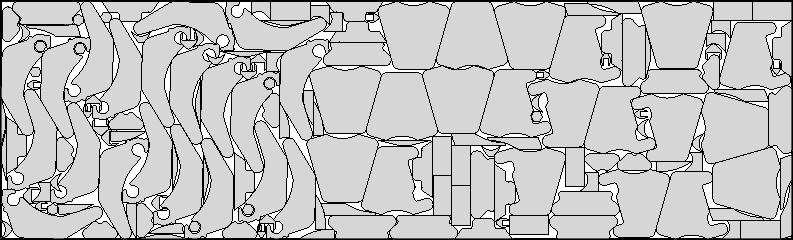
\includegraphics[height=\subfigheight]{final_best_gardeyn7_svg-raw.pdf}
        \caption{\texttt{GARDEYN7}}
    \end{subfigure}
    \hfill
    \begin{subfigure}[t]{0.33\linewidth}
        \centering
        %\includesvg[inkscapelatex=false, height=\subfigheight]{new_instances/inverted/final_best_gardeyn8.svg}
        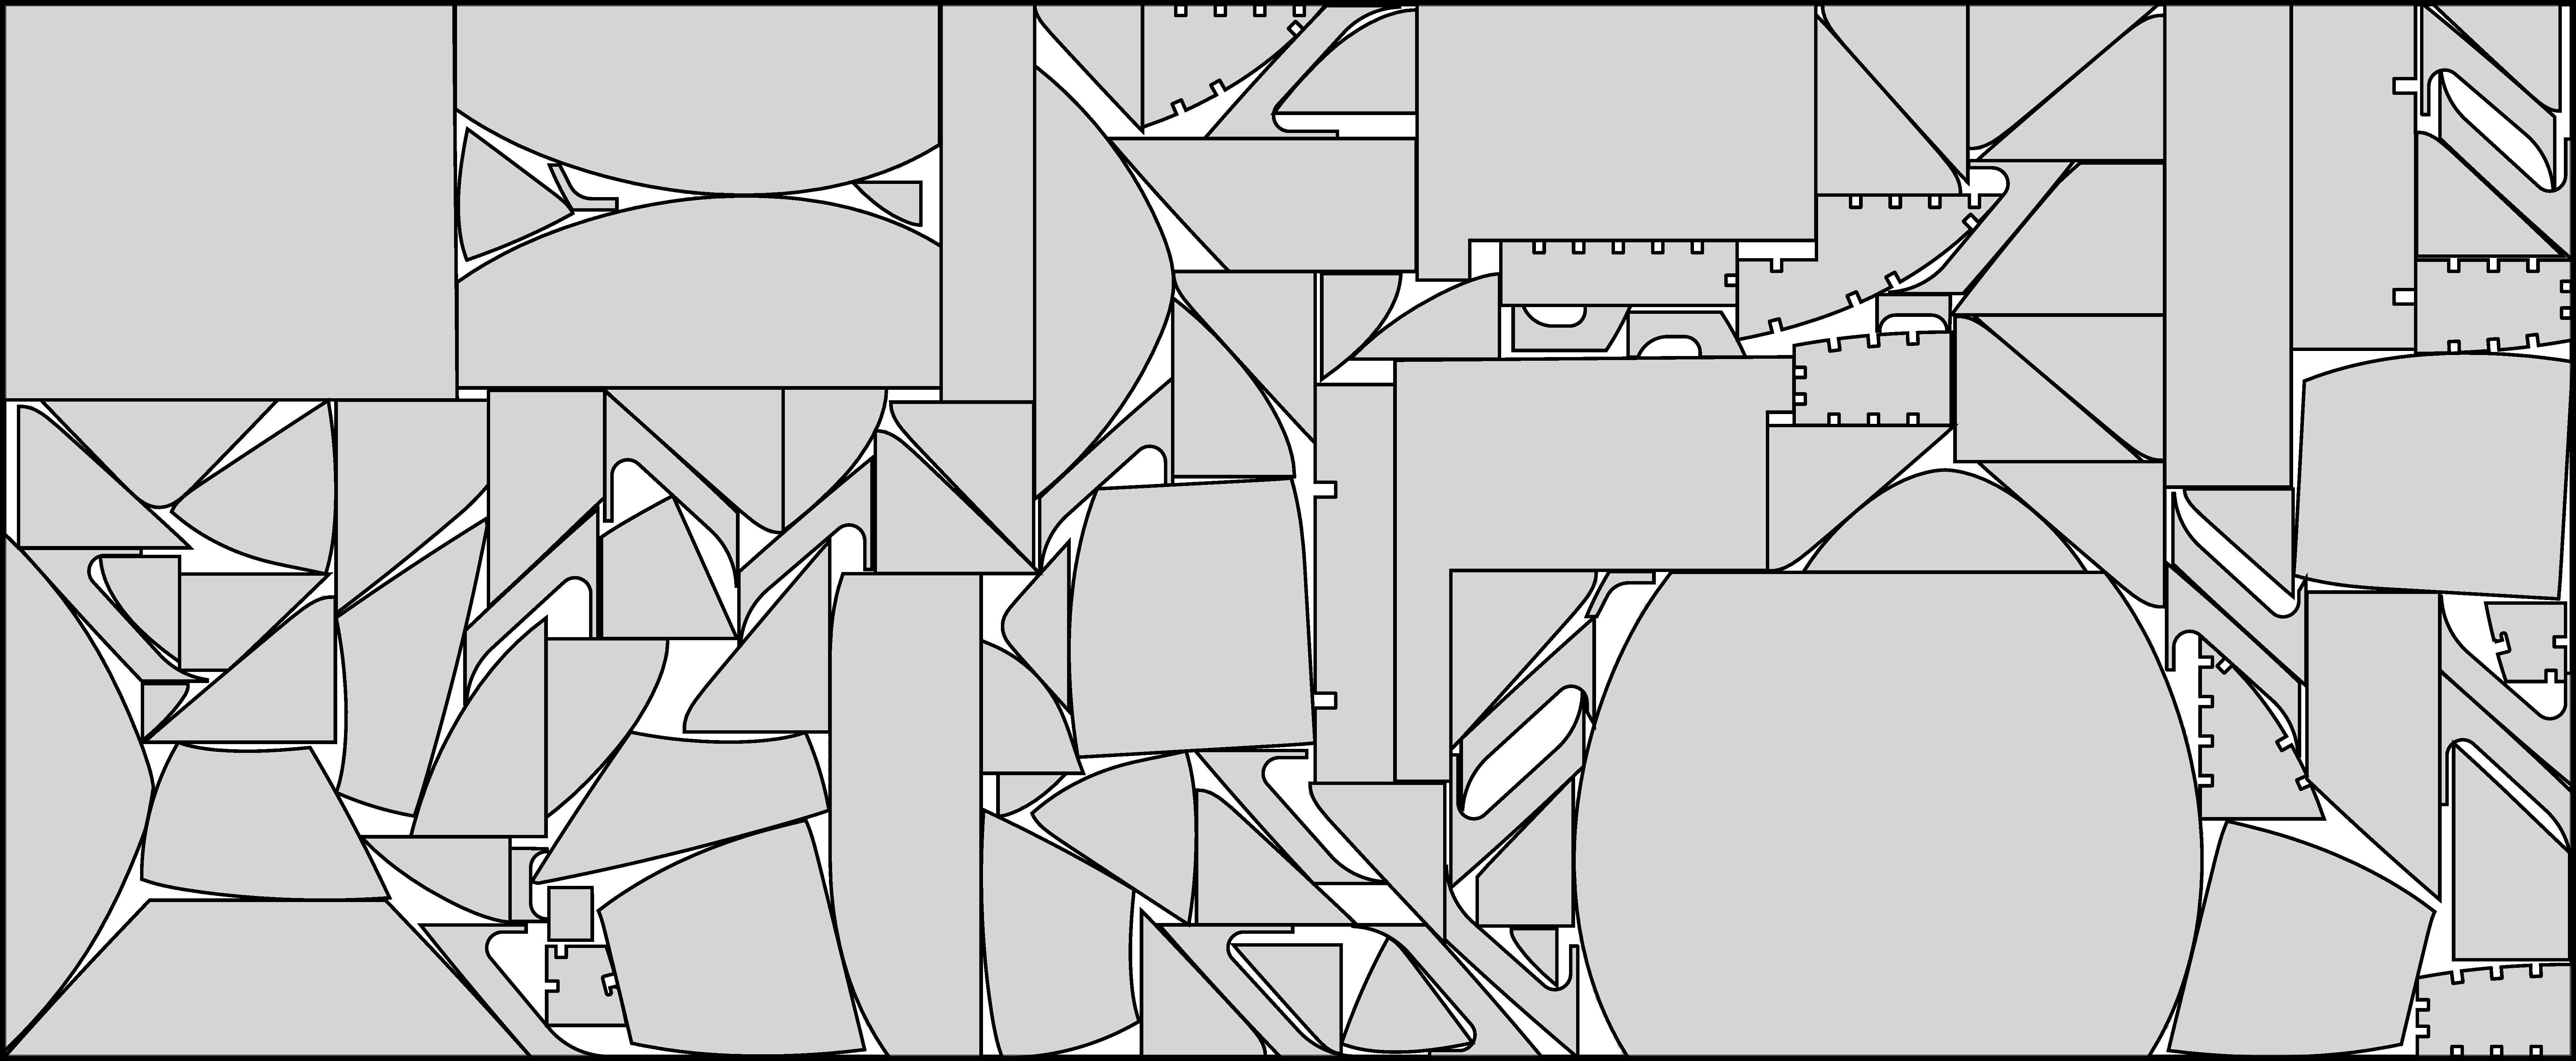
\includegraphics[height=\subfigheight]{final_best_gardeyn8_svg-raw.pdf}
        \caption{\texttt{GARDEYN8}}
    \end{subfigure}
    \hfill
    \begin{subfigure}[t]{0.2\linewidth}
        \hfill
        %\includesvg[inkscapelatex=false, height=\subfigheight]{new_instances/inverted/final_best_gardeyn9.svg}
        
\includegraphics[height=\subfigheight]{final_best_gardeyn9_svg-raw.pdf}
        \caption{\texttt{GARDEYN9}}
    \end{subfigure}

    \caption{Ten new benchmark instances for the 2DISPP. The visualizations are solutions produced by \texttt{sparrow}.}
    \label{fig:new_instances}
\end{figure}